\section{Numerical Simulations}

\subsection{Environmental flux}

SPENVIS uses the AP-8/AE-8 model to simulate the trapped proton and electron models, which can simulate the fluxes during solar maximum and minimum.

For the worst-case simulation the solar maximum is considered. 

For the protons the number of trapped protons is higher during solar minimum due to the increased scale height caused by the increased UV radiation from the sun, but only for lower altitudes, for this orbit the difference between solar minimum and maximum for the proton flux is negligible, which is not the case for the electrons.

In figures \ref{fig:e_map} and \ref{fig:p_map} the integrated fluxes are displayed over the orbit in GEI mode.

The highes proton fluxes are expected at perigee, while for the electron flux the highes flux is expected during crossing of the radiation belts (c.f. fig. \ref{fig:e_wmap}).

\begin{figure}[!htbp]
  \centering
  \begin{minipage}[b]{0.45\textwidth}
    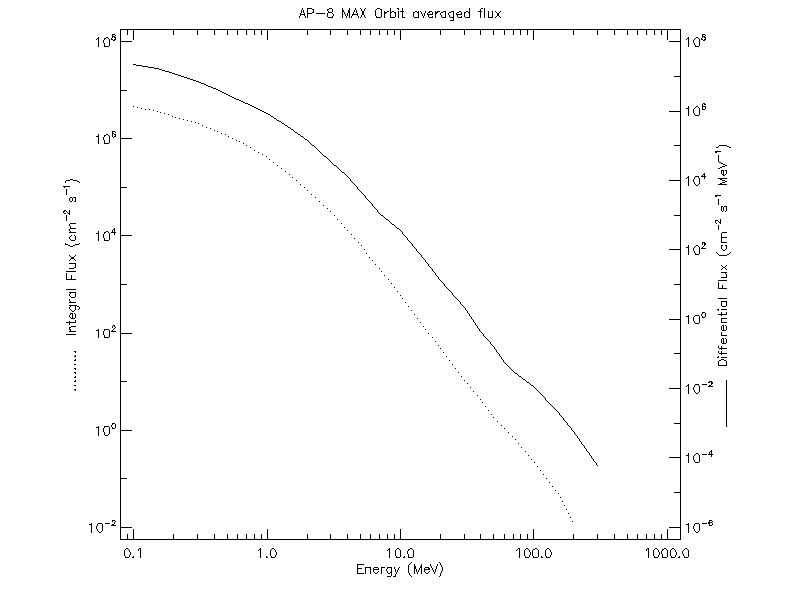
\includegraphics[width=\textwidth]{spenvis/max_prot}
    \caption{Proton Flux}
    \label{fig:p_flux}
  \end{minipage}
  \hfill
  \begin{minipage}[b]{0.45\textwidth}
    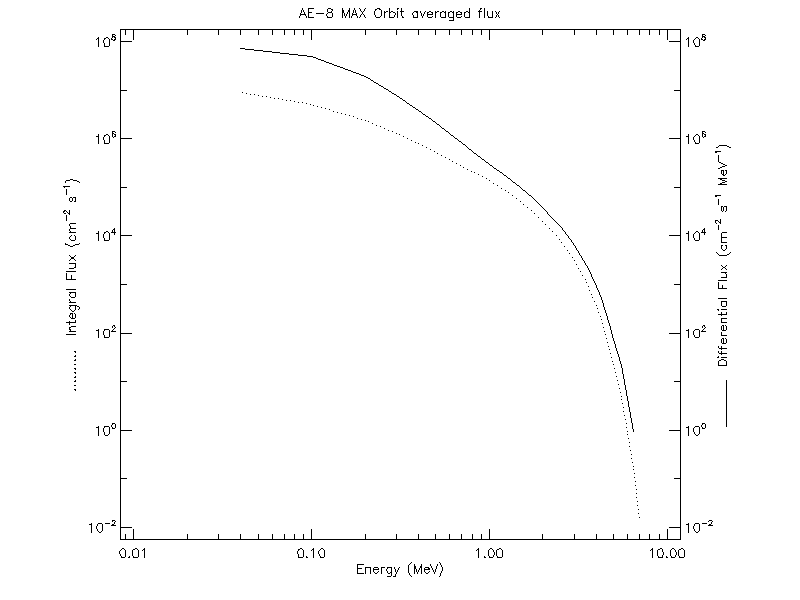
\includegraphics[width=\textwidth]{spenvis/max_elec}
    \caption{Electron Flux}
    \label{fig:e_flux}
  \end{minipage}
\end{figure}

\begin{figure}[!htbp]
  \centering
  \begin{minipage}[b]{0.45\textwidth}
    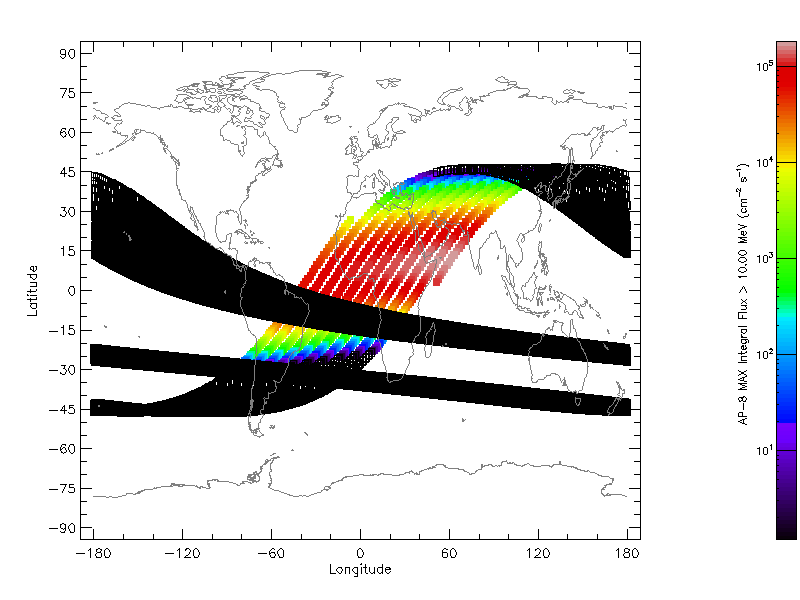
\includegraphics[width=\textwidth]{spenvis/proton_map}
    \caption{Proton Flux greater than 1 MeV}
    \label{fig:p_map}
  \end{minipage}
  \hfill
  \begin{minipage}[b]{0.45\textwidth}
    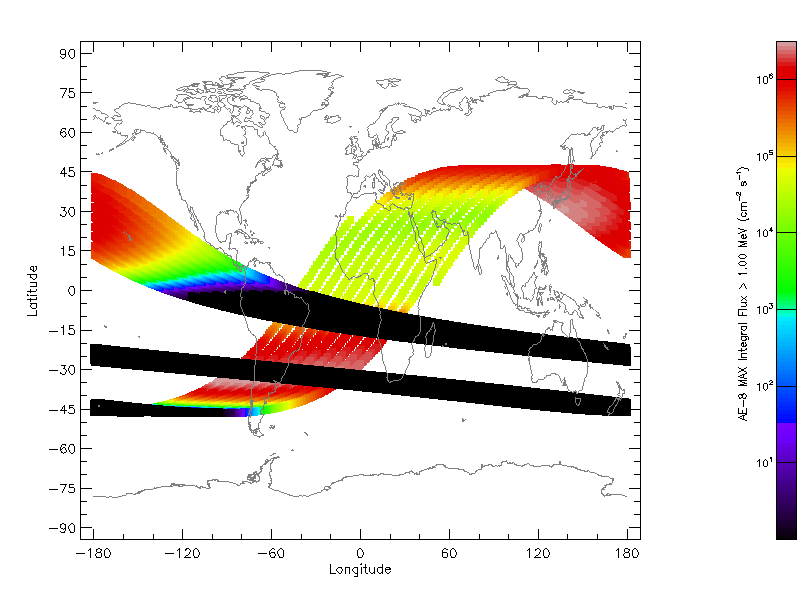
\includegraphics[width=\textwidth]{spenvis/electron_map}
    \caption{Electron Flux greater than 1 MeV}
    \label{fig:e_map}
  \end{minipage}
\end{figure}

\begin{figure}[h]
	\centering
	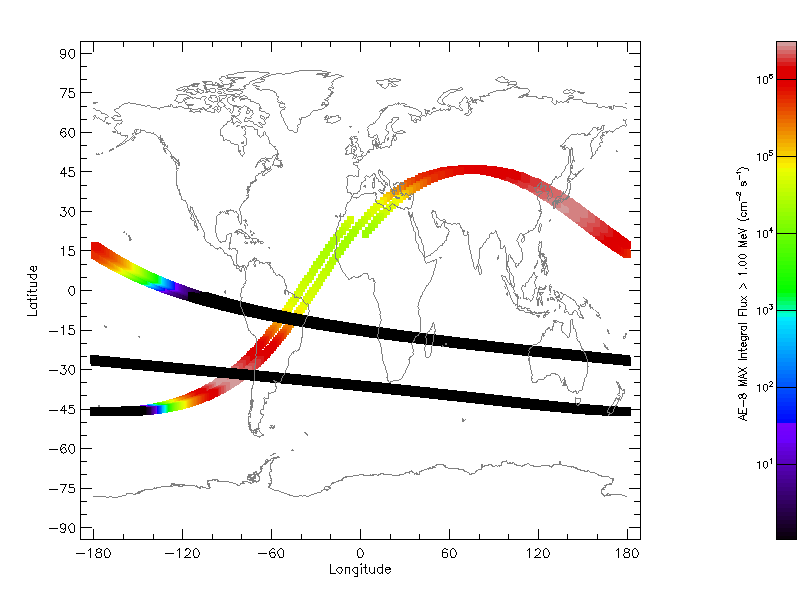
\includegraphics[width=\linewidth-5em]{spenvis/electron_wmap}
		\caption{Electron Flux World map}
		 \label{fig:e_wmap}
\end{figure}

\subsection{Lifetime and Performance Degradation}

The satellite is using Azur 3G28 solar cells, with an EOL power of 95\% of the BOL power \citep{evans:labInstructions}.

Using SPENVIS' MC-SCREAM for solar cells, it was determined that the shielding thickness should be around 230 \textmu m which leaves an EOL powerloss of 3.3\%.

\subsection{Total Dose and Shielding}

The satellite is using a memory device which can withstand a total radiation dose of 25 Krad before failure.

With 1mm of shielding the memory device exceeds its maximum radiation dose with a total dose of 1.5 Mrad, which is about 62 times the maximum allowed dose.

To achieve a maximum dose of 25 Krad or less the shielding has to be increased to a minimum of 5.1mm, which will lead to a maximum dose of 26 Krad.


\begin{figure}[h]
	\centering
	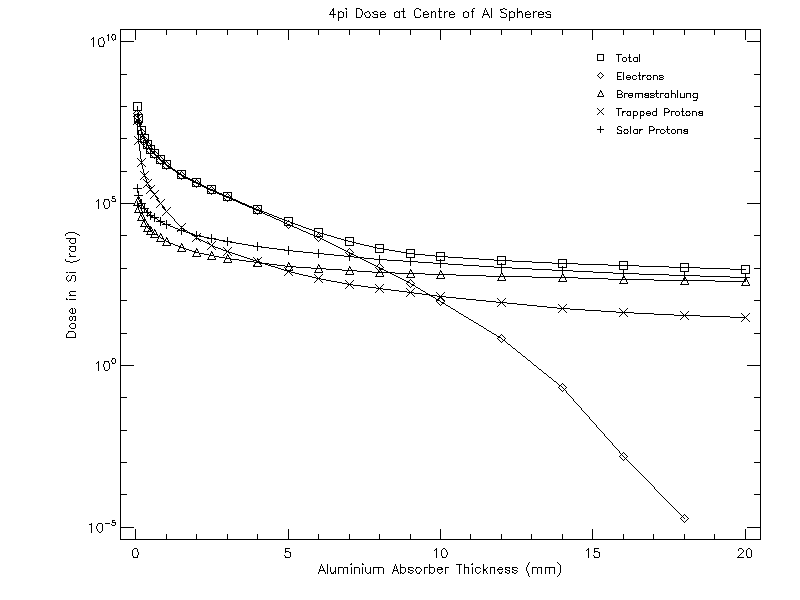
\includegraphics[width=\linewidth-5em]{spenvis/memory_rad}
		\caption{Dose received vs. Shielding in mm}
		 \label{fig:rad_memory}
\end{figure}
\subsection{Single Event Upsets}

\subsection{Linear Energy Transfer (LET) Spectrum}

\subsection{Cross Section and Components Characteristics}

\subsection{SEU Estimation}